\documentclass{article}\usepackage[]{graphicx}\usepackage[]{color}
%% maxwidth is the original width if it is less than linewidth
%% otherwise use linewidth (to make sure the graphics do not exceed the margin)
\makeatletter
\def\maxwidth{ %
  \ifdim\Gin@nat@width>\linewidth
    \linewidth
  \else
    \Gin@nat@width
  \fi
}
\makeatother

\definecolor{fgcolor}{rgb}{0.345, 0.345, 0.345}
\newcommand{\hlnum}[1]{\textcolor[rgb]{0.686,0.059,0.569}{#1}}%
\newcommand{\hlstr}[1]{\textcolor[rgb]{0.192,0.494,0.8}{#1}}%
\newcommand{\hlcom}[1]{\textcolor[rgb]{0.678,0.584,0.686}{\textit{#1}}}%
\newcommand{\hlopt}[1]{\textcolor[rgb]{0,0,0}{#1}}%
\newcommand{\hlstd}[1]{\textcolor[rgb]{0.345,0.345,0.345}{#1}}%
\newcommand{\hlkwa}[1]{\textcolor[rgb]{0.161,0.373,0.58}{\textbf{#1}}}%
\newcommand{\hlkwb}[1]{\textcolor[rgb]{0.69,0.353,0.396}{#1}}%
\newcommand{\hlkwc}[1]{\textcolor[rgb]{0.333,0.667,0.333}{#1}}%
\newcommand{\hlkwd}[1]{\textcolor[rgb]{0.737,0.353,0.396}{\textbf{#1}}}%

\usepackage{framed}
\makeatletter
\newenvironment{kframe}{%
 \def\at@end@of@kframe{}%
 \ifinner\ifhmode%
  \def\at@end@of@kframe{\end{minipage}}%
  \begin{minipage}{\columnwidth}%
 \fi\fi%
 \def\FrameCommand##1{\hskip\@totalleftmargin \hskip-\fboxsep
 \colorbox{shadecolor}{##1}\hskip-\fboxsep
     % There is no \\@totalrightmargin, so:
     \hskip-\linewidth \hskip-\@totalleftmargin \hskip\columnwidth}%
 \MakeFramed {\advance\hsize-\width
   \@totalleftmargin\z@ \linewidth\hsize
   \@setminipage}}%
 {\par\unskip\endMakeFramed%
 \at@end@of@kframe}
\makeatother

\definecolor{shadecolor}{rgb}{.97, .97, .97}
\definecolor{messagecolor}{rgb}{0, 0, 0}
\definecolor{warningcolor}{rgb}{1, 0, 1}
\definecolor{errorcolor}{rgb}{1, 0, 0}
\newenvironment{knitrout}{}{} % an empty environment to be redefined in TeX

\usepackage{alltt}
\usepackage{geometry}
\geometry{verbose,tmargin=2cm,bmargin=2cm,lmargin=2.5cm,rmargin=2.5cm}
\IfFileExists{upquote.sty}{\usepackage{upquote}}{}
\begin{document}





\title{Estimating the undiagnosed fraction and total number of PLWHA in WA state: Backcalculation from testing history data}
\author{Martina Morris and Jeanette Birnbaum}
\maketitle

\section{WA State Estimates for All HIV Cases}
``Total-weighted" refers to the sum of separate estimates for MSM vs non-MSM, whereas ``Total" refers to estimates made pooling all cases at once. The former allows the cases with missing testing history to draw upon data from those in their transmission group, rather than the whole population.

\begin{knitrout}\footnotesize
\definecolor{shadecolor}{rgb}{0.969, 0.969, 0.969}\color{fgcolor}\begin{figure}[h]


{\centering 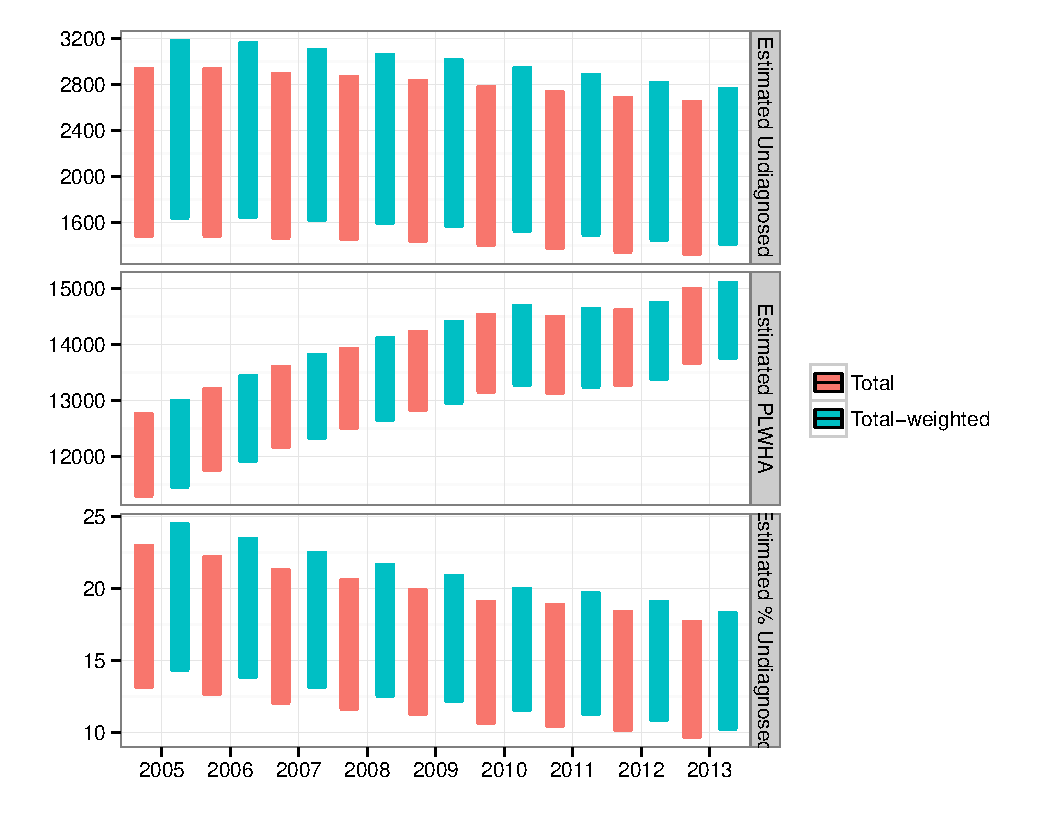
\includegraphics[width=\maxwidth]{figure/minimal-all-WA} 

}

\caption[Estimated undiagnosed cases, total PLWHA (known PLWHA + undiagnosed cases) and the undiagnosed fraction (undiagnosed cases as a percent of total PLWHA)]{Estimated undiagnosed cases, total PLWHA (known PLWHA + undiagnosed cases) and the undiagnosed fraction (undiagnosed cases as a percent of total PLWHA). Ranges represent a base case and an upper bound case\label{fig:all-WA}}
\end{figure}


\end{knitrout}


\pagebreak
\section{WA State Estimates for MSM vs non-MSM Cases}
MSM refers to MSM and MSM/IDU transmission groups, and non-MSM to all other cases. 

\subsection{Years 2005-2013}
\begin{knitrout}\footnotesize
\definecolor{shadecolor}{rgb}{0.969, 0.969, 0.969}\color{fgcolor}\begin{figure}[h]


{\centering 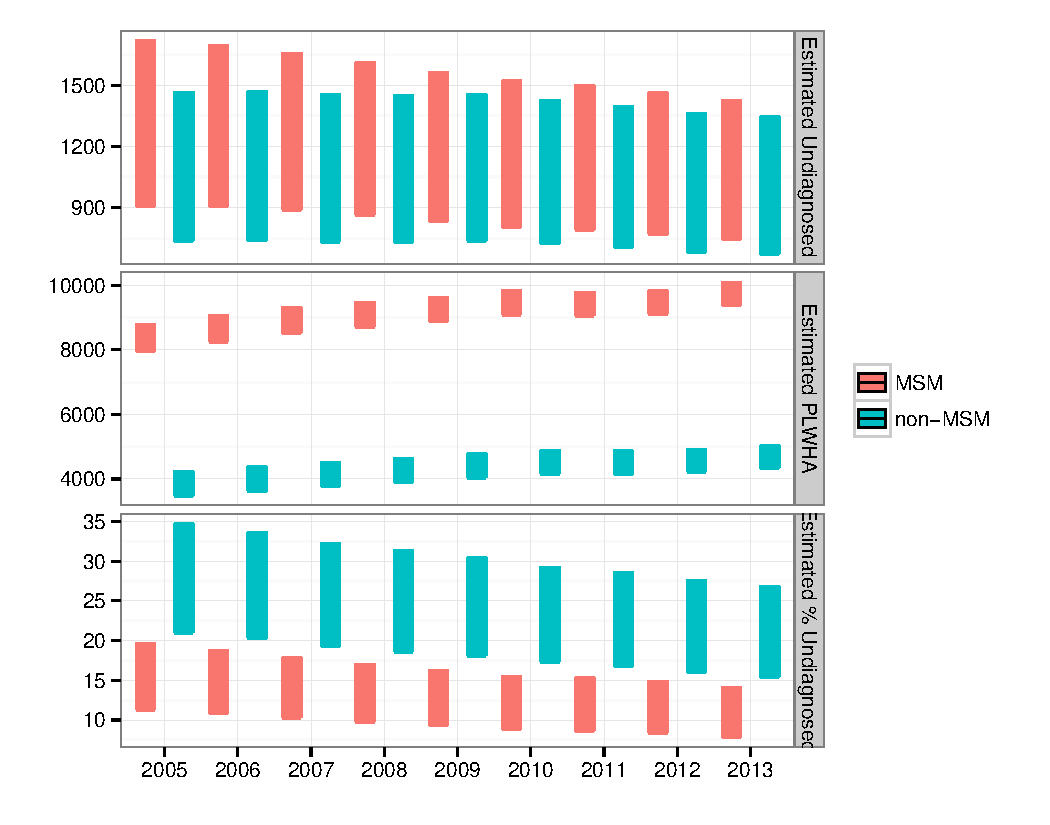
\includegraphics[width=\maxwidth]{figure/minimal-WA-MSM} 

}

\caption[For MSM and non-MSM in WA, estimated undiagnosed cases, total PLWHA (known PLWHA + undiagnosed cases) and the undiagnosed fraction (undiagnosed cases as a percent of total PLWHA)]{For MSM and non-MSM in WA, estimated undiagnosed cases, total PLWHA (known PLWHA + undiagnosed cases) and the undiagnosed fraction (undiagnosed cases as a percent of total PLWHA). Ranges represent a base case and an upper bound case\label{fig:WA-MSM}}
\end{figure}


\end{knitrout}


\pagebreak
\subsection{2013 Estimates Including Missing Data}
In all other figures, the ranges reflect a base case and upper bound estimate derived only using cases who answered the testing history question, ``Have you ever had a negative test?", as ``Yes" or ``No." In the figure below, we include two additional estimates, a base case and an upper bound, that incorporated the cases who had missing data for the testing history question. The estimates that exclude and include missing data are labeled (Observed) and (Missing) respectively. (Note: in a previous report, Upper Bound was called Worst Case). 
\begin{knitrout}\footnotesize
\definecolor{shadecolor}{rgb}{0.969, 0.969, 0.969}\color{fgcolor}\begin{figure}[h]


{\centering 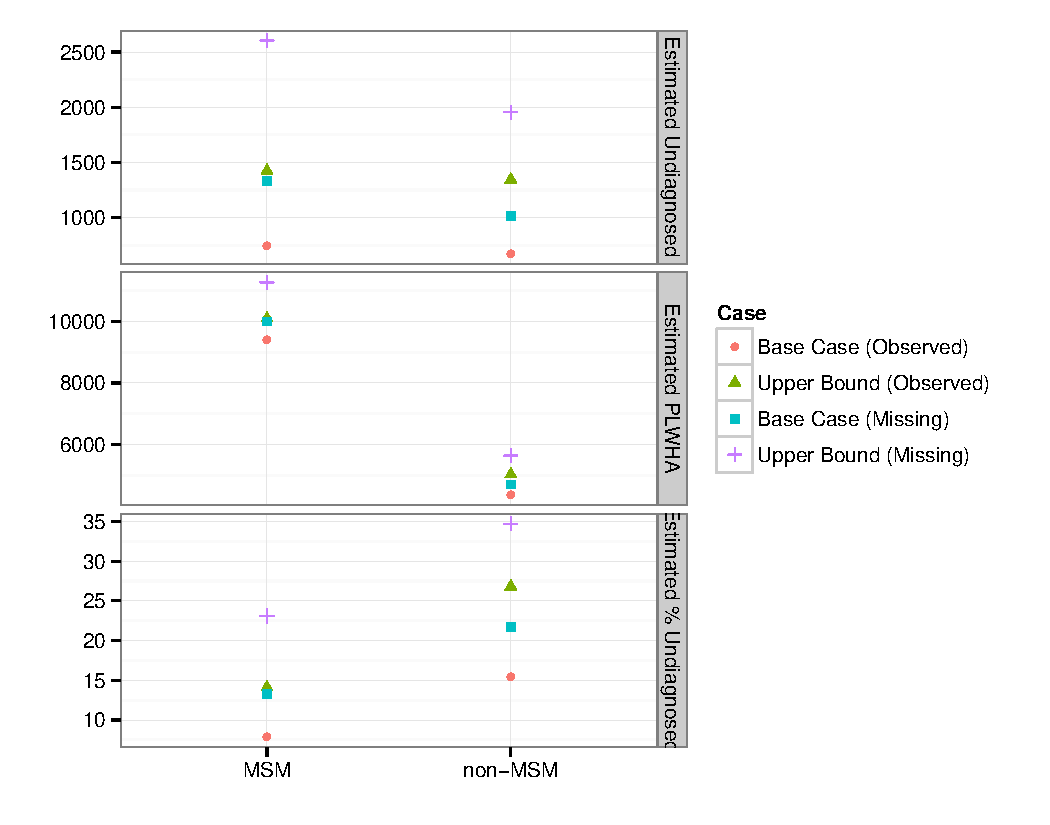
\includegraphics[width=\maxwidth]{figure/minimal-WA-MSM-allcases} 

}

\caption[For MSM and non-MSM in WA in 2013, estimated undiagnosed cases, total PLWHA (known PLWHA + undiagnosed cases) and the undiagnosed fraction (undiagnosed cases as a percent of total PLWHA)]{For MSM and non-MSM in WA in 2013, estimated undiagnosed cases, total PLWHA (known PLWHA + undiagnosed cases) and the undiagnosed fraction (undiagnosed cases as a percent of total PLWHA). The four points represent a base case and an upper bound case for Observed, when missing data were excluded, and Missing, when missing data were included\label{fig:WA-MSM-allcases}}
\end{figure}


\end{knitrout}


\pagebreak
\section{WA State and KC Estimates for MSM}
MSM refers to MSM and MSM/IDU transmission groups only.

\begin{knitrout}\footnotesize
\definecolor{shadecolor}{rgb}{0.969, 0.969, 0.969}\color{fgcolor}\begin{figure}[h]


{\centering 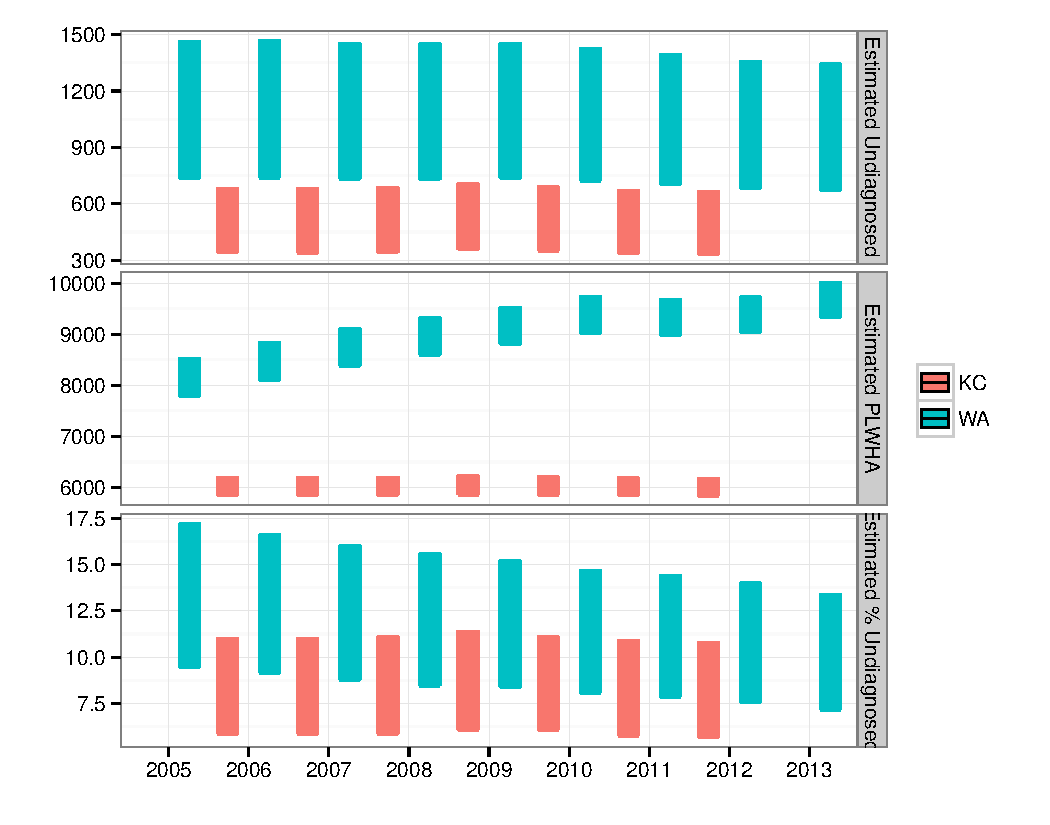
\includegraphics[width=\maxwidth]{figure/minimal-MSM} 

}

\caption[Among MSM in WA and KC only, estimated undiagnosed cases, total PLWHA (known PLWHA + undiagnosed cases) and the undiagnosed fraction (undiagnosed cases as a percent of total PLWHA)]{Among MSM in WA and KC only, estimated undiagnosed cases, total PLWHA (known PLWHA + undiagnosed cases) and the undiagnosed fraction (undiagnosed cases as a percent of total PLWHA). Ranges represent a base case and an upper bound case\label{fig:MSM}}
\end{figure}


\end{knitrout}


\end{document}


